\chapter{Технологическая часть}

\section{Выбор средств реализации}

Для реализации приложения был выбран высокоуровненый язык Java, поскольку он поддерживает объектно-ориентированную парадигму программирования и позволяет писать приложения, запускаемые в любой системе с помощью виртуальной Java-машины~\cite{java}.

Для хранения информации, связанной с предметной областью, будет использована клиент-серверная СУБД. В таблице~\ref{dms_comp} представлен сравнительный анализ наиболее популярных клиент-серверных СУБД.

\begin{center}
	\begin{threeparttable}
		\captionsetup{justification=raggedright,singlelinecheck=off}
		\caption{\label{dms_comp}Сравнительный анализ клиент-серверных СУБД}
		\centering
		\begin{tabular}{|c|c|c|c|}
			\hline
			\multirow{2}{*}{Критерий} & \multicolumn{3}{|c|}{СУБД} \\
			\cline{2-4}
			& PostgreSQL~\cite{postgresql} & MongoDB~\cite{mssql} & Oracle~\cite{oracle} \\
			\hline
			\specialcell{Тип} & Реляционная & Документоориентированная & Реляционная \\
			\hline
			\specialcell{Открытый\\исходный код} & + & + & - \\
			\hline
			\specialcell{Операционная\\система\\сервера} & \specialcell{Windows\\Unix\\Linux\\OS X} & \specialcell{Windows\\Unix\\Linux} & \specialcell{Windows\\Linux\\OS X} \\
			\hline
			\specialcell{Поддержка\\SQL} & + & - & + \\
			\hline
			\specialcell{Поддержка\\триггеров} & + & - & + \\
			\hline
		\end{tabular}
	\end{threeparttable}
\end{center}

Для работы с базой данных была выбрана система PostgreSQL, поскольку она имеет открытый исходный код, доступна под наиболее популярные операционные системы и имеет поддержку триггеров.

Приложение должно обеспечивать хранение логов в отдельной базе данных. В качестве СУБД будет использована СУБД временных рядов, поскольку, в отличие от других систем, она оптимизирована для быстрого приема запросов: скорость загрузки данных не уменьшается со временем и остается стабильной~\cite{timedb}. В таблице~\cite{time_dms_comp} представлен сравнительный анализ наиболее популярных СУБД временных рядов.

\begin{center}
	\begin{threeparttable}
		\captionsetup{justification=raggedright,singlelinecheck=off}
		\caption{\label{time_dms_comp}Сравнительный анализ СУБД временных рядов}
		\centering
		\begin{tabular}{|c|c|c|c|}
			\hline
			\multirow{2}{*}{Критерий} & \multicolumn{3}{|c|}{СУБД} \\
			\cline{2-4}
			& InfluxDB~\cite{influxdb} & Prometheus~\cite{prometheus} & Graphite~\cite{graphite} \\
			\hline
			\specialcell{Тип по\\способу\\доступа} & Клиент-серверная & Клиент-серверная & Клиент-серверная \\
			\hline
			\specialcell{Открытый\\исходный код} & + & + & + \\
			\hline
			\specialcell{Операционная\\система\\сервера} & \specialcell{Linux\\OS X} & \specialcell{Windows\\Linux} & \specialcell{Linux\\Unix} \\
			\hline
			\specialcell{Поддерживаемые\\типы данных} & Числа и строки & Числа & Числа \\
			\hline
		\end{tabular}
	\end{threeparttable}
\end{center}

Для логирования была выбрана СУБД InfluxDB, поскольку она является клиент-серверной и поддерживает такие типы данных, как числа и строки. Для логирования СУБД PostgreSQL в InfluxDB был выбран плагин Telegraf~\cite{telegraf}.

В качестве СУБД для кэширования информации и организации очереди запросов предлагается использовать встраиваемые системы <<ключ-значение>>. В таблице~\ref{in_dms_comp} представлен сравнительный анализ наиболее популярных встраиваемых СУЬД <<ключ-значение>>.

\begin{center}
	\begin{threeparttable}
		\captionsetup{justification=raggedright,singlelinecheck=off}
		\caption{\label{in_dms_comp}Сравнительный анализ встраиваемых СУБД <<ключ-значение>>}
		\centering
		\begin{tabular}{|c|c|c|}
			\hline
			\multirow{2}{*}{Критерий} & \multicolumn{2}{|c|}{СУБД} \\
			\cline{2-3}
			& Memcached~\cite{memcached} & Redis~\cite{redis} \\
			\hline
			\specialcell{Открытый исходный код} & + & + \\
			\hline
			\specialcell{Операционная система} & \specialcell{Windows\\Unix\\Linux\\OS X} & \specialcell{Windows\\Linux\\OS X} \\
			\hline
			\specialcell{Поддержка скриптов} & - & + \\
			\hline
			\specialcell{Поддержка транзакций} & - & + \\
			\hline
		\end{tabular}
	\end{threeparttable}
\end{center}

Для кеширования и организации очереди запросов была выбрана СУБД Redis, поскольку она поддерживает пользовательские скрипты и транзакции.

\section[Описание сущностей и ограничений целостности базы данных]{Описание сущностей и ограничений целостности\\базы данных}

В листингах~\ref{users_lst}--\ref{bet_enclosures_lst} представлены описания сущностей и ограничений целостности базы данных.
\begin{figure}[H]
	\begin{lstlisting}[label=users_lst,caption=Описание сущности users,language=Caml]
create table if not exists users
(
    login text primary key,
    hashed_pswd text not null check (hashed_pswd != ''),
    role int not null check (role <= 2 and role >= 0)
);
	\end{lstlisting}
\end{figure}
\begin{figure}[H]
	\begin{lstlisting}[label=referees_lst,caption=Описание сущности referees,language=Caml]
create table if not exists referees
(
    id int primary key,
    first_name text not null check (first_name != ''),
    second_name text not null check (second_name != ''),
    third_name text,
    birth_date date not null,
    country text not null check (country != '')
);
	\end{lstlisting}
\end{figure}
\begin{figure}[H]
	\begin{lstlisting}[label=players_lst,caption=Описание сущности players,language=Caml]
create table if not exists players
(
    id int primary key,
    first_name text not null check (first_name != ''),
    second_name text not null check (second_name != ''),
    third_name text,
    birth_date date not null,
    country text not null check (country != ''),
    raiting int not null check (raiting >= 0)
);
	\end{lstlisting}
\end{figure}
\begin{figure}[H]
	\begin{lstlisting}[label=moves_lst,caption=Описание сущности moves,language=Caml]
create table if not exists moves
(
    id int serial primary key,
    figure int not null check (figure >= 0 and figure <= 5),
    start_cell text not null check (start_cell != ''),
    end_cell text not null check (end_cell != '')
);
	\end{lstlisting}
\end{figure}
\begin{figure}[H]
	\begin{lstlisting}[label=games_lst,caption=Описание сущности games,language=Caml]
create table if not exists games
(
    id int primary key,
    round int not null check (round >= 1 and round <= 8),
    duration int,
    number int not null check (number > 0),
    result int check (result >= 0 and result <= 2),
    date date,
    referee_id int references referees (id) on delete cascade,
    first_player_id int references players (id) on delete cascade,
    second_player_id int references players (id) on delete cascade
);

alter table games add constraint first_player_id check (first_player_id != second_player_id);
alter table games add constraint second_player_id check (first_player_id != second_player_id);
	\end{lstlisting}
\end{figure}
\begin{figure}[H]
	\begin{lstlisting}[label=bets_lst,caption=Описание сущности bets,language=Caml]
create table if not exists bets
(
    id int primary key,
    type int not null check (type >= 0 and type <= 2),
    condition text check (condition = ''),
    coefficient real check (coefficient > 1),
    status int not null check (status >= 0 and status <= 2),
    game_id int references games (id) on delete cascade
);
	\end{lstlisting}
\end{figure}
\begin{figure}[H]
	\begin{lstlisting}[label=game_moves_lst,caption=Описание сущности game\_moves,language=Caml]
create table if not exists game_moves
(
    game_id int references games (id) on delete cascade,
    move_id int references moves (id) on delete cascade,
    number int not null check (number > 0),
    comment text
);
	\end{lstlisting}
\end{figure}
\begin{figure}[H]
	\begin{lstlisting}[label=bet_enclosures_lst,caption=Описание сущности bet\_enclosures,language=Caml]
create table if not exists bet_enclosures
(
    bet_id int references bets (id) on delete cascade,
    enclosure_id int references bets (id) on delete cascade
);

alter table bet_enclosures add constraint bet_id check (bet_id != enclosure_id);
alter table bet_enclosures add constraint enclosure_id check (bet_id != enclosure_id);
	\end{lstlisting}
\end{figure}

\section{Реализация триггеров}

В листингах~\ref{remove_next_moves_lst}--\ref{update_raitings_lst2} представлены реализованные триггеры и функции, необходимые для их выполнения.
\begin{figure}[H]
	\begin{lstlisting}[label=remove_next_moves_lst,caption=Триггер удаления ходов из шхатманой партии,language=Caml]
create or replace function remove_next_moves() returns trigger as
  $remove_next_moves_trigger$
    begin
      delete from game_moves where move_id >= old.move_id and game_id = old.game_id;
      delete from moves where id not in (select move_id from game_moves);
      return null;
    end;
  $remove_next_moves_trigger$
language plpgsql;

create trigger remove_next_moves_trigger
after delete on game_moves
when (pg_trigger_depth() = 0)
execute function remove_next_moves();
	\end{lstlisting}
\end{figure}
\begin{figure}[H]
	\begin{lstlisting}[label=update_bets_status_lst,caption=Триггер проверки выполнения условий ставок,language=Caml]
create or replace function update_bets_status() returns trigger as 
  $update_bets_status_trigger$
    declare
      bet record;
        express_status int;
        express record;
      begin 
        for bet in select * from bets
          loop
            if bet.type = 0 then
              if bet.game_id = old.id then
                if is_main_line(bet.condition) then
                  if is_achieved(bet.condition, old.result) then
                    update bets set status = 1 where id = bet.id;
                  else
                    update bets set status = 2 where id = bet.id;
                  end if;
                end if;
              end if;
            elsif bet.type = 1 then
              express_status := new_express_status(bet, game);
              if express_status != bet.status then
                update bets set status = express_status where id = bet.id;
              end if;
            elsif bet.type = 2 then
              for express in
                select enclosure_id as id, type, condition, coefficient, status, game_id
                from game_moves gm join bets b on enclosure_id = id
                where bet_id = bet.id
              loop
                express_status := new_express_status(express, old);
                if express_status != express.status then
                  update bets set status = express_status where id = express.id;
                end if;
              end loop;
            end if;
          end loop;
        return null;
      end;
  $update_bets_status_trigger$
language plpgsql;

create trigger update_bets_status_trigger
after update of result on games
for each row
execute function update_bets_status();
	\end{lstlisting}
\end{figure}
\begin{figure}[H]
	\begin{lstlisting}[label=update_raitings_lst1,caption=Триггер обновления рейтинга игроков (начало),language=Caml]
create or replace function update_raitings() returns trigger as
  $update_raitings_trigger$
    declare
      prob1 real;
      prob2 real;
      raiting1 int;
      raiting2 int;
      new_raiting1 int;
      new_raiting2 int;
      delta1 int;
      delta2 int;
      raiting_delta1 int;
      raiting_delta2 int;
    begin
      select raiting into raiting1 from players where id = new.first_player_id;
      select raiting into raiting2 from players where id = new.second_player_id;
      if (raiting1 > raiting2) then
        select weak_player_win_prob(raiting1 - raiting2) into prob2;
        prob1 := 1.0 - prob2;
      else
        select weak_player_win_prob(raiting2 - raiting1) into prob1;
        prob2 := 1.0 - prob1;
      end if;
      if new.result = 0 then
        delta1 := 0.5 - prob1;
        delta2 := 0.5 - prob2;
      elsif new.result = 1 then
        delta1 := 1 - prob1;
        delta2 := -1 * prob2;
      else
        delta1 := -1 * prob1;
        delta2 := 1 - prob2;
      end if;
      if raiting1 <= 2400 then
        raiting_delta1 := delta1 * 20;
      else
        raiting_delta1 := delta1 * 10;
      end if;
      if raiting2 <= 2400 then
        raiting_delta2 := delta2 * 20;
      else
        raiting_delta2 := delta2 * 10;
      end if;
      if raiting_delta1 > 700 then
        raiting_delta1 := 700;
      end if;
	\end{lstlisting}
\end{figure}
\begin{figure}[H]
	\begin{lstlisting}[label=update_raitings_lst2,caption=Триггер обновления рейтинга игроков (конец),language=Caml]
      if raiting_delta2 > 700 then
        raiting_delta2 = 700;
      end if;
      update players set raiting = raiting + raiting_delta1 where id = new.first_player_id;
      update players set raiting = raiting + raiting_delta2 where id = new.second_player_id;
      return new;
    end;
  $update_raitings_trigger$
language plpgsql;

create trigger update_raitings_trigger
after update of result on games
for each row 
execute function update_raitings();
	\end{lstlisting}
\end{figure}

\section{Описание ролевой модели на уровне базы данных}

В листингах~\ref{unauthorized_lst}--\ref{bookmaker_lst} представлено описание ролевой модели на уровне базы данных.

\begin{figure}[H]
	\begin{lstlisting}[label=unauthorized_lst,caption=Описание роли неаторизованного пользователя,language=Caml]
create user unauthorized with encrypted password 'unauthorized';
grant select on users to unauthorized;
	\end{lstlisting}
\end{figure}
\begin{figure}[H]
	\begin{lstlisting}[label=administrator_lst,caption=Описание роли администратора,language=Caml]
create user administrator with encrypted password 'administrator';
grant select, update, delete, insert on bet_enclosures to administrator;
grant select, update, delete, insert on bets to administrator;
grant select, update, delete, insert on bet_enclosures to administrator;
grant select, update, delete, insert on game_moves to administrator;
grant select, update, delete, insert on games to administrator;
grant select, update, delete, insert on moves to administrator;
grant select, update, delete, insert on players to administrator;
grant select, update, delete, insert on referees to administrator;
grant select, update, delete, insert on users to administrator;
	\end{lstlisting}
\end{figure}
\begin{figure}[H]
	\begin{lstlisting}[label=spectator_lst,caption=Описание роли наблюдателя,language=Caml]
create user spectator with encrypted password 'spectator';
grant select on referees, players to spectator;
grant select, update, delete, insert on games to spectator;
grant select, update, delete, insert on moves to spectator;
grant select, update, delete, insert on game_moves to spectator;
	\end{lstlisting}
\end{figure}
\begin{figure}[H]
	\begin{lstlisting}[label=bookmaker_lst,caption=Описание роли букмекера,language=Caml]
create user bookmaker with encrypted password 'bookmaker';
grant select on referees, players, games, moves, game_moves to bookmaker;
grant select, update, delete, insert on bets to bookmaker;
grant select, update, delete, insert on bet_enclosures to bookmaker;
	\end{lstlisting}
\end{figure}

\section{Пользовательский интерфейс}

Для разработки графического пользовательского интерфейса была использована библиотека Java Swing~\cite{swing}. На рисунках~\ref{unauthorized_ui}--\ref{bookmaker_ui} представлен графический пользовательский интерфейс приложения.
\begin{figure}[H]
	\centering
	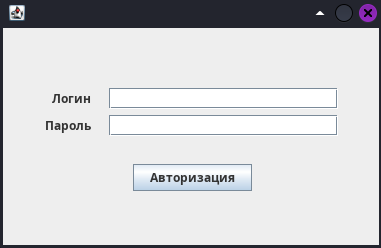
\includegraphics[width=0.5\linewidth]{unauthorized_ui}
	\caption{Графический интерфейс неавторизованного пользователя}
	\label{unauthorized_ui}
\end{figure}
\begin{figure}[H]
	\centering
	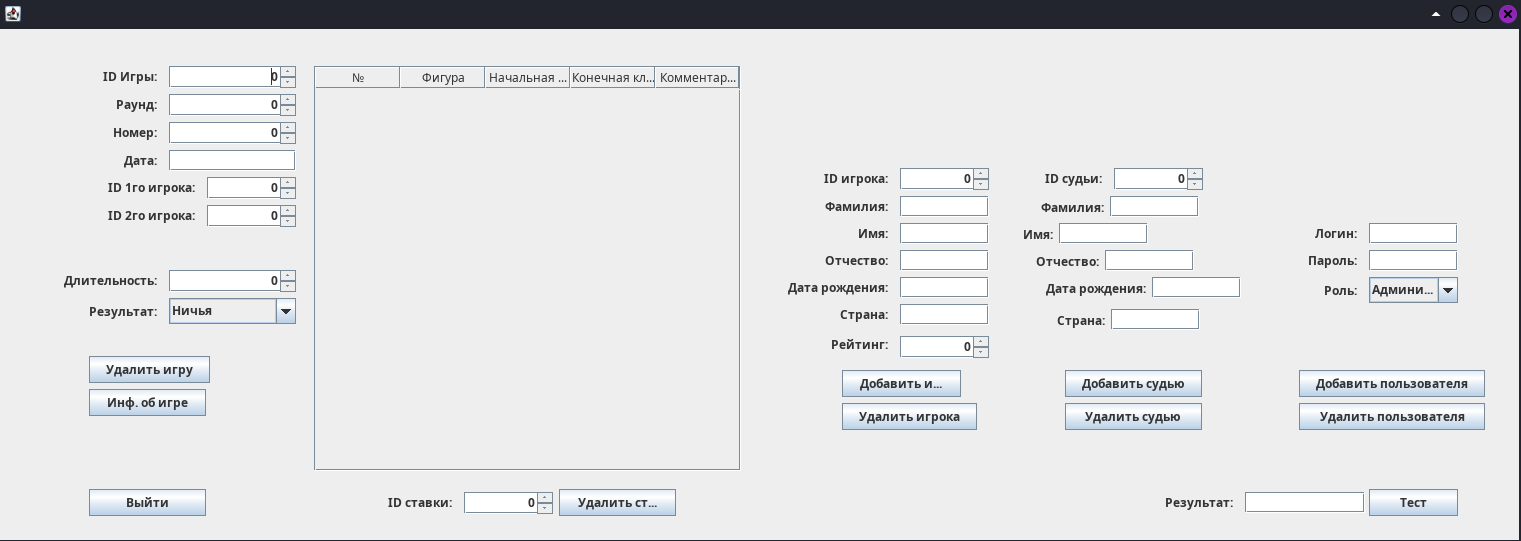
\includegraphics[width=\linewidth]{admin_ui}
	\caption{Графический интерфейс администратора}
	\label{admin_ui}
\end{figure}
\begin{figure}[H]
	\centering
	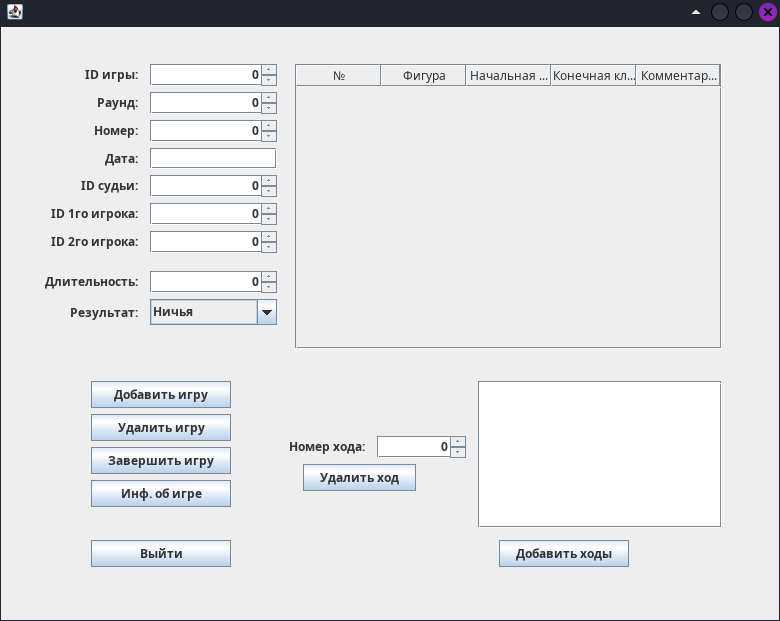
\includegraphics[width=0.7\linewidth]{spectator_ui}
	\caption{Графический интерфейс наблюдателя}
	\label{spectator_ui}
\end{figure}
\begin{figure}[H]
	\centering
	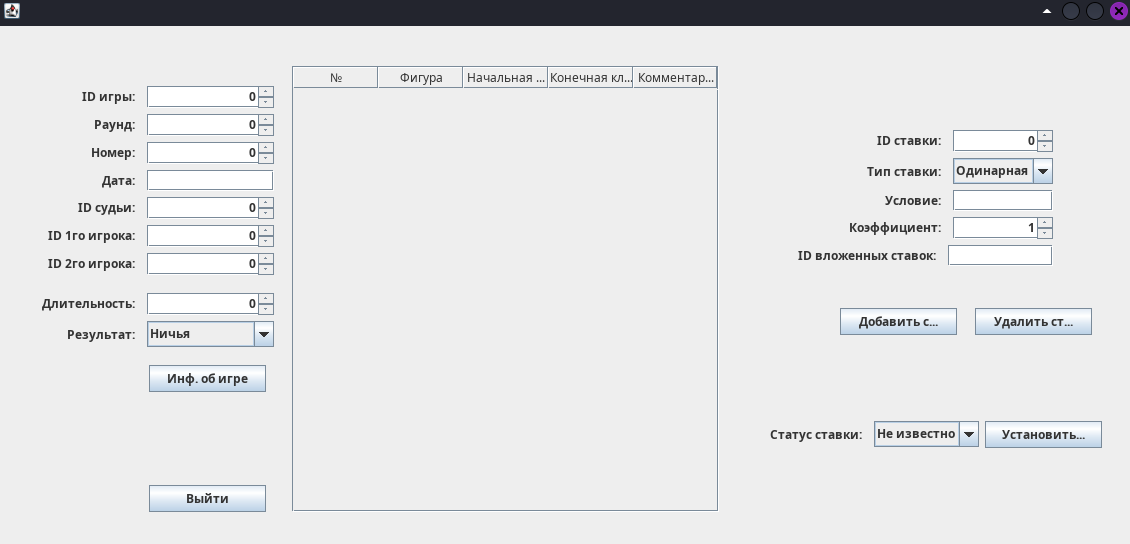
\includegraphics[width=\linewidth]{bookmaker_ui}
	\caption{Графический интерфейс букмекера}
	\label{bookmaker_ui}
\end{figure}

\section*{Вывод}

В технологическом разделе были проанализированы и выбраны средства реализации приложения и базы данных. Были описаны триггеры, пользователи и ограничения целостности базы данных. Был разработан графический пользовательский интерфейс приложения.

\clearpage
